%设置整个文档字体大小,纸张
\documentclass[UTF8,a4paper,10pt]{ctexart}

%设置页面格式
\usepackage[left=2.50cm, right=2.50cm, top=2.50cm, bottom=2.50cm]{geometry}

%可以用于禁止浮动体浮动
\usepackage{float}

%表格竖线连续化
\usepackage{makecell}
\newcommand\toprule{\Xhline{.08em}}
\newcommand\midrule{\Xhline{.05em}}
\newcommand\bottomrule{\Xhline{.08em}}

%!\I 就可以代替| 来画表格了
\def\I{\vrule width1.2pt}

%缩进支持
\usepackage{indentfirst}

%可以插入代码
\usepackage{listings}
%语法高亮支持
\usepackage{xcolor}
%代码格式
\definecolor{dkgreen}{rgb}{0,0.6,0}
\definecolor{gray}{rgb}{0.5,0.5,0.5}
\definecolor{mauve}{rgb}{0.58,0,0.82}
\lstset{ %
	%language=Python,	% 编程语言,这里可以不用先设置,用到的时候再设置
	breaklines,	%自动折行
	%extendedchars=false	%解决代码跨页时,章节标题,页眉等汉字不显示的问题
	keepspaces=false,  
	%tabsize=4 	%设置tab空格数
	showspaces=false,  %不显示空格
	showtabs=false,  
	showstringspaces=true, 
	numbers=left, 
	basicstyle=\footnotesize, 
	numberstyle=\tiny, 
	numbersep=5pt, 
	keywordstyle= \color{ blue!70},	%关键字颜色
	commentstyle= \color{red!50!green!50!blue!50},	%注释颜色 
	frame=shadowbox,	 % 边框格式:阴影效果
	rulesepcolor= \color{ red!20!green!20!blue!20} ,
	escapeinside=``,	 % 英文分号中可写入中文
	xleftmargin=2em,xrightmargin=2em, aboveskip=1em,	%设置页边距
	framexleftmargin=2em
}

%设置章节标题左对齐
\CTEXsetup[format={\Large\bfseries}]{section} 

%超链接颜色,会影响文中中引用的字体颜色
\usepackage[colorlinks,linkcolor=black,anchorcolor=blue,citecolor=black]{hyperref}

%自定义页眉、页脚
\usepackage{fancyhdr}  %使用fancyhdr包自定义页眉页脚
\pagestyle{fancy}
%\pagestyle{plain}%没有页眉,页脚放页数
\renewcommand{\headrulewidth}{0.5pt}
\renewcommand{\footrulewidth}{0.4pt}
\lhead{}
\chead{}
\rhead{}
\lfoot{}
\cfoot{\thepage}
\rfoot{}

%可以使用插图图片相关
\usepackage{caption}
\usepackage{graphicx, subfig}

\begin{document}



%表头部分
\centerline{\LARGE\textbf{Operational Statistics for SAR Imagery Report}} 
\vspace{1cm}

\qquad\qquad\setlength{\parindent}{1em}{\textbf{Author:}}{\kaishu \textbf{Zhenyu Li}}\qquad\qquad\qquad\qquad\qquad\qquad\qquad\quad {\textbf{2019.10.5}}
\renewcommand\arraystretch{1.5}


\section{Experiment Environment}
Win10,RStdio

\section{Some Statistical Distribution}
During the entire course of Synthetic Aperture Rader(SAR), I was exposed to some statistical distribution like K distribution, Gamma distribution etc. And simulated them by using matlab, python, and R. In this section, I'd like to introduce each distribution function and image.

\subsection{Exponential Distribution}
The distribution function is defined as:
\begin{equation}
f(x) = \frac{1}{\sigma^2}e^\frac{-x}{\sigma^2}
\end{equation}

\begin{figure}[htb] \center
	\includegraphics[width=5cm]  {1.png}
	\includegraphics[width=5cm]  {2.png}
	\caption{ Exponential distribution with means 1/2,1 and 2(red,black,blue,resp.) of Cartesian coordinates(left) and logarithmic coordinates(right)} 
\end{figure}
\par The distribution with means 1/2,1 and 2 is plotted as figure 1.

\subsection{Gamma Distribution}
After that, here come the Gamma distribution which is defined as:
\begin{equation}
f_Z(z,L,\sigma^2) = \frac{L^L}{\sigma^{2L}\Gamma(L)}z^{L-1}exp\{-Lz/\sigma^2\}
\end{equation}
\\\par Where $\Gamma(v)$ is the Gamma function given by $\Gamma(v) = \int_{R_+} {t^{v-1}e^{-t}dt}$

\begin{figure}[htb] \center
	\includegraphics[width=5cm]  {3.png}
	\includegraphics[width=5cm]  {4.png}
	\caption{ Gamma distribution of Cartesian coordinates(left) and logarithmic coordinates(right)} 
\end{figure}
\par Figure 2 is shown that three  cases of the Gamma distribution with uni-tary mean and shape parameters (Looks) equal to 1 (the Exponen-tial distribution), 3 and 8,then convert it to logarithmic coordinates.

\subsection{K Distribution}
This distribution function is defined as :
\begin{equation}
f_Z(z,\alpha,\lambda,L) = \frac{2{\lambda}L}{\Gamma(\alpha)\Gamma(L)}{\lambda}Lz^{\frac{\alpha+L}{2}-1}K_{\alpha-L}(2\sqrt{\lambda{Lz}})
\end{equation}
\par Where $\alpha>0$ measures the roughness,$\lambda>0$ is a scale parame-ter, and $K_v$ is the modified Bessel function of order $v$ . This special function is given by $K_v(z) = \int_0^\infty {e^{-z}cosh(vt)dt}$.
\par For this function, figure 3 shows the distribution with unitary mean ( $\alpha \in { 1,3,8 }$ in red, blue, black, resp.),then convert it to logarithmic coordinates.

\begin{figure}[htb] \center
	\includegraphics[width=5cm]  {5.png}
	\includegraphics[width=5cm]  {6.png}
	\caption{K distribution of Cartesian coordinates(left) and logarithmic coordinates(right)} 
\end{figure}

\subsection{$G_0$ Distribution}
The $G_0$ distribution function is defined as:
\begin{equation}
f_Z(z,\alpha,\gamma,L) = \frac{L^L\Gamma(L-\alpha)}{\gamma^\alpha\Gamma(L)\Gamma(-\alpha)}\frac{Z^{l-1}}{(\gamma+Lz)^{{L-\alpha}^\prime}}
\end{equation}
\par Figure 4 shows the distribution with unitary mean ( $\alpha \in { -1.5,-3,-8 }$ in red, blue, black, resp.),then convert it to logarithmic coordinates.

\begin{figure}[htb] \center
	\includegraphics[width=5cm]  {7.png}
	\includegraphics[width=5cm]  {8.png}
	\caption{ $G_0$ distribution of Cartesian coordinates(left) and logarithmic coordinates(right)} 
\end{figure}

\section{SAR Image Analysis}
In this section, I analysis an image from the given data.Figure 5 shows that the image I choosed.And figure 6 shows that the histogram.

\begin{figure}[htb] \center
	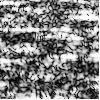
\includegraphics[width=7cm]  {a.png}
	\caption{ } 
\end{figure}
\begin{figure}[htb] \center
	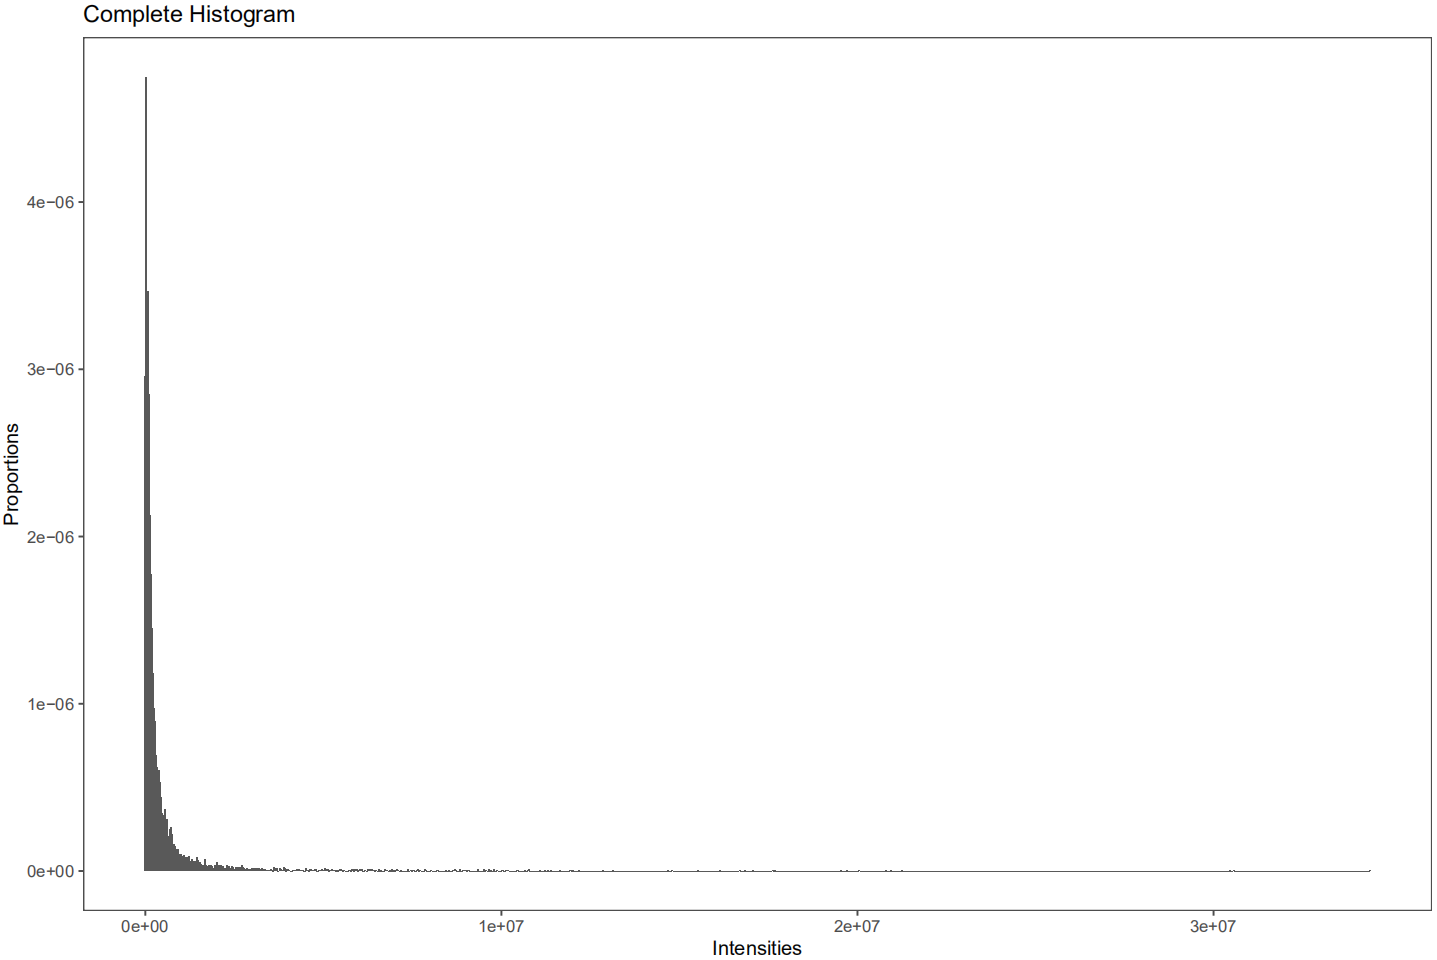
\includegraphics[width=10cm]  {b.png}
	\caption{ } 
\end{figure}
\end{document}
